\subsection*{Step 2.3}
\label{sec:2.3}
To determine the values of $a_i$ and $b_i$ for $i \in \{1,2,3,4\}$ that minimizes the squared area between $f$ and $\hat{f}$, 
\begin{align}
    \int_{0}^{\bar{u}_{d}}\left(f\left(u_{\mathrm{d}}\right)-\hat{f}\left(u_{\mathrm{d}}\right)\right)^{2} d u_{\mathrm{d}} \label{eq:2.3cost}
\end{align}
a new PWA function of $f(u_d)-\hat{f}(u_d)$ has been created where the regions of $f(u_d)$ have been synced with the four functions of $\hat{f}(u_d)$. This created four separate minimization problems which have been minimized with \textit{fmincon()}. Equailty constraints were used, so that the functions have the same function value at the boundary. The steps to arrive at the given solutions are:
\begin{enumerate}
    \item Approximate the first part, results in $a_1$ and $b_1$.
    \item Compute $\hat{f}(u_d)$ at the end of the first part (at $u_d$ = 5).
    \item Solve for the second part $(5\leq u_d<6.5)$ with an equality constraint $a_1+5b_1 = a_2+5b_2$.
    \item Repeat this for all parts, with the appropriate bounds and parameters
\end{enumerate}
The optimal variables are shown in table \ref{tab:2.3table}, and figure \ref{fig:part23} shows $\hat{f}(u_d)$.\\
\begin{table}[h]
    \centering
    \caption{The optimal variables $a_i$, $b_i$}
    \begin{tabular}{c|c|c|c}
    \hline
         $a_1$ &  1.8133 & $b_1$ & 3.488 \\
         $a_2$ &  -83.647 & $b_2$ & 20.58  \\
         $a_3$ &  110.08 & $b_3$ & -9.2246 \\
         $a_4$ &  -212.98 & $b_4$ & 20.144   
    \end{tabular}
    
    \label{tab:2.3table}
    \end{table}
A Matlab script \ref{} has been created to perform this PWA approximation, which can be examined for further explanation.
\begin{figure}[ht]
    \centering
    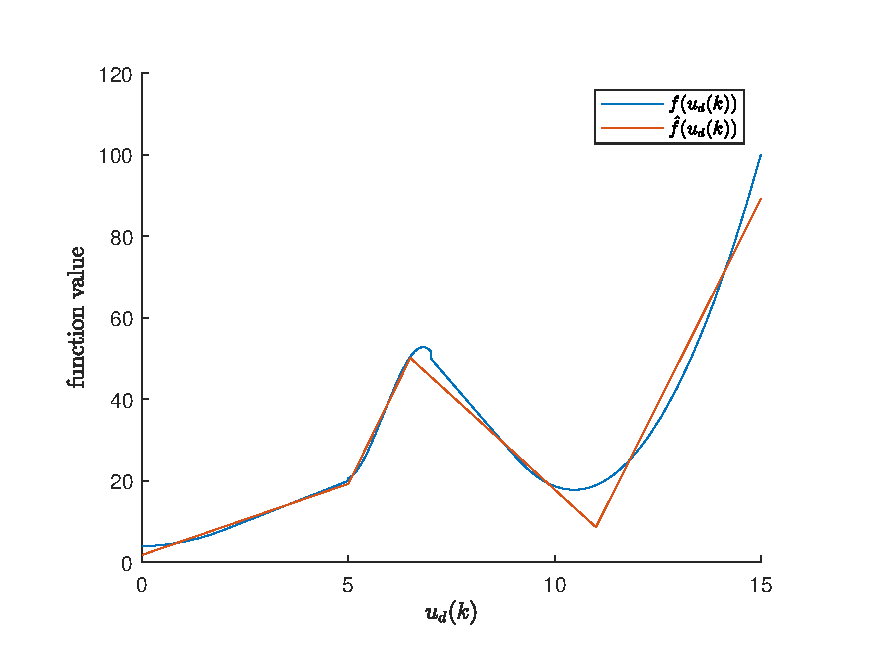
\includegraphics[width=0.8\textwidth]{Latex/images/step23.pdf}
    \caption{PWA approximation comparison}
    \label{fig:part23}
\end{figure}
